\documentclass{beamer}
%\documentclass[handout]{beamer}
%\setbeameroption{show notes}


% Think backwards: what do you want people to remember from your talk?
% Don’t say everything.
% Simplify.


% For parts #1 to #9, we expect a fair distribution of the slides among the topics, while taking into account your progress (e.g., a 3rd year PhD student should report on a strong Evaluation / Validation, while a 1st year PhD student is more expected to provide a clear view on the state-of-the-art and the foreseen contribution(s) ). We highly recommend you to have a look to last year feedback made by Jacques and Ernesto [1] on the quality of your presentation and their weaknesses.
% 
% For part #10, we expect you to think about how your work can integrate in the LEDA laboratory. If you do not know what LEDA is about, ask Gwen. Gwen has kindly prepared a short document (attached) that summarises the availability of devices in LEDA and the way they are already integrated. This part (as the others) is mandatory and you are expected to propose something valuable for the group.

\usecolortheme[named=blue]{structure}

\mode<presentation>
{
  \usetheme{Warsaw}
  \setbeamercovered{transparent}
}

\usepackage{listings}
%\lstset{basicstyle=\scriptsize}

\title[{Repairing Bugs in Conditional Expressions}]{Repairing~Bugs~in~Conditional~Expressions}
\author[Favio DeMarco]{Favio~DeMarco}
\institute[U.B.A. - INRIA]{Universidad de Buenos Aires - INRIA}
\date[08/28/2013]{August 28th, 2013}
\subject{Computational Sciences}

\begin{document}

  \frame
  {
\begin{quote}
    Take nothing on its looks; take everything on evidence. There's no better rule.
\end{quote}    
– Charles Dickens, ``Great Expectations.''
  }

\frame
  {
    \titlepage
  }

  \frame
  {
    \frametitle{Context}
    \framesubtitle{So far, the Universe is winning.}
    \begin{quote}
    Bug fixing continues to be a mostly manual, time consuming, and therefore expensive activity in software development.
    \end{quote}
    Hoang Duong Thien Nguyen et al, ``SemFix: Program Repair via Semantic Analysis''
}

 \begin{frame}[fragile]
    \frametitle{Case study}
      \framesubtitle{Commons Math - MathUtils class}
\begin{lstlisting}[escapeinside=\[\]]
public static int gcd(int u, int v) {
  if ([\textbf{u * v == 0}]) {
    return (Math.abs(u) + Math.abs(v));
  }
...
\end{lstlisting}
\end{frame}

 \begin{frame}[fragile]
    \frametitle{Case study}
      \framesubtitle{Commons Math}
        \begin{lstlisting}[escapeinside=\[\]]
assertEquals([\textbf{3 * (1$<<$15)}]
        , gcd(3 * (1<<20), 9 * (1<<15)));
	\end{lstlisting}
\end{frame}

 \begin{frame}[fragile]
    \frametitle{Case study}
      \framesubtitle{Commons Math}
        \begin{lstlisting}[escapeinside=\[\]]
public static int gcd(int u, int v) {
    if ([\textbf{(u == 0) $||$ (v == 0)}]) {
        return (Math.abs(u) + Math.abs(v));
    }
    // ...
}
	\end{lstlisting}
\end{frame}

{
\usebackgroundtemplate{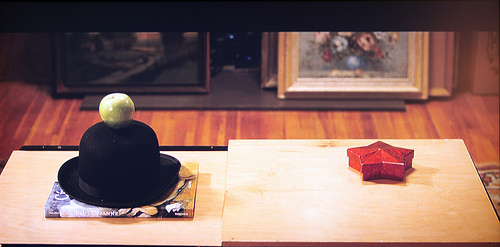
\includegraphics[width=\paperwidth]{500daysofsummer}}%
  \frame
  {
    \frametitle{State of the art}
  }
}

  \frame
  {
    \frametitle{State of the art}
    SemFix: Program Repair via Semantic Analysis
\begin{itemize}
\item Statement ranking (Tarantula) $\rightarrow$
\item Symbolic Execution (KLEE) $\rightarrow$
\item Repair Constraint $\rightarrow$  Program Synthesis (SOLFP\footnote{Synthesis of Loop-free Programs} -paper-)
\end{itemize}
 }


  \frame
  {
    \frametitle{State of the art}
    GenProg: A Generic Method for Automatic Software Repair
    
Claire Le Goues, ThanhVu Nguyen, Stephanie Forrest, Westley Weimer
  }

  \frame
  {
    \frametitle{State of the art}
    ClearView, AutoFix-E, Gopinath et al, Pachika.
  }

  \frame
  {
    \frametitle{Problems}
    Unwillingness to share code.
  }

  \frame
  {
    \frametitle{Problems}
    \framesubtitle{Test quality}
   \begin{quote}
    Quality is free, but only to those who are willing to pay heavily for it.
   \end{quote}
   – Tom DeMarco, Peopleware
   
   
%    0 != up_sep
%    
%    or (adding a border case test)
%    
%    !((up_sep <= inhibit) && ((down_sep == 100) || (inhibit < 1)))
%    
%    !=
%    
%    ((0 != inhibit) ? (up_sep + 100) : up_sep) > down_sep
   
  }
 
  \frame
  {
    \frametitle{Limitations}
    Resources (time, code monkeys, knowledge, tools, etc.).
  }

  \frame
  {  
    \frametitle{Contributions}
      \framesubtitle{Process}
\begin{itemize}
\item Statement ranking (GZoltar)  $\rightarrow$
\item Ad hoc code manipulation and values capturing (OGCBPS\footnote{Oracle-Guided Component-Based Program Synthesis} -paper-) $\rightarrow$
\item Repair Constraint  $\rightarrow$
\item Program Synthesis (SOLFP\footnote{Synthesis of Loop-free Programs} -paper-)
\end{itemize}
}


  \frame
  {
    \frametitle{Experimental methodology}
    Seeded and wild bugs.
  }
  
  \frame
  {
    \frametitle{Evaluation / Validation}
    Generated patches vs. reality.
  }
  
  \frame
  {
    \frametitle{Perspectives}
    
  }
  
  \frame
  {
    \frametitle{Conclusion}
    
  }

  \frame
  {
    \frametitle{Contribution}
    
  }
  
 \frame
  {
    \frametitle{Can't and shouldn't.}
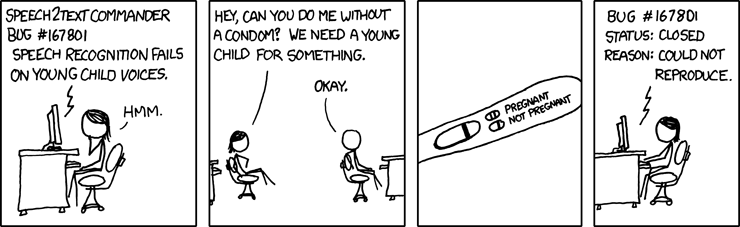
\includegraphics[width=.8\paperwidth]{cnr}

}

%Programming today is a race between software engineers striving to build bigger and better idiot-proof programs, and the Universe trying to produce bigger and better idiots. So far, the Universe is winning.
% Rick Cook, The Wizardry Compiled


 \begin{frame}[fragile]
    \frametitle{Case study}
      \framesubtitle{Commons Math - MathUtils class}
\begin{lstlisting}[escapeinside=\[\]]
411: public static int gcd(int u, int v) {
412:   if ([\textbf{u * v == 0}]) {
413:     return (Math.abs(u) + Math.abs(v));
414:   }
...
\end{lstlisting}
\end{frame}

 \begin{frame}[fragile]
    \frametitle{Case study}
      \framesubtitle{Commons Math}
        \begin{lstlisting}[escapeinside=\[\]]
assertEquals([\textbf{3 * (1$<<$15)}]
        , gcd(3 * (1<<20), 9 * (1<<15)));
	\end{lstlisting}
\end{frame}

 \begin{frame}[fragile]
    \frametitle{Case study}
      \framesubtitle{Statement ranking (GZoltar)}
\begin{verbatim}
MathUtils:413 Suspiciousness 0.23570226039551587
MathUtils:431 Suspiciousness 0.1543033499620919
\end{verbatim}
...
\begin{verbatim}
MathUtils:460 Suspiciousness 0.11322770341445956
MathUtils:412 Suspiciousness 0.11180339887498948
\end{verbatim}
\end{frame}

 \begin{frame}[fragile]
    \frametitle{Case study}
      \framesubtitle{Ad hoc code manipulation and values capturing (OGCBPS -paper-)}
\begin{lstlisting}[escapeinside=\[\]]
411: public static int gcd(int u, int v) {
412:   if ([\textbf{true}]) {
413:     return (Math.abs(u) + Math.abs(v));
414:   }
...
\end{lstlisting}
\end{frame}

  \frame
  {  
  \frametitle{Case study}
      \framesubtitle{Repair Constraint}
\begin{equation*}
 (u=0\wedge v=0 \Rightarrow output=true) \wedge
\end{equation*}
\begin{equation*}
 (u=0\wedge v=55 \Rightarrow output=true) \wedge 
\end{equation*}
\begin{equation*}
...
\end{equation*}
\begin{equation*}
 (u=77\wedge v=55 \Rightarrow output=false)
\end{equation*}
}

 \begin{frame}[fragile]
    \frametitle{Case study}
      \framesubtitle{Commons Math}
        \begin{lstlisting}[escapeinside=\[\]]
public static int gcd(int u, int v) {
    if ([\textbf{(u == 0) $||$ (v == 0)}]) {
        return (Math.abs(u) + Math.abs(v));
    }
    // ...
}
	\end{lstlisting}
\end{frame}


\end{document}
